\documentclass[1p]{elsarticle_modified}
%\bibliographystyle{elsarticle-num}

%\usepackage[colorlinks]{hyperref}
%\usepackage{abbrmath_seonhwa} %\Abb, \Ascr, \Acal ,\Abf, \Afrak
\usepackage{amsfonts}
\usepackage{amssymb}
\usepackage{amsmath}
\usepackage{amsthm}
\usepackage{scalefnt}
\usepackage{amsbsy}
\usepackage{kotex}
\usepackage{caption}
\usepackage{subfig}
\usepackage{color}
\usepackage{graphicx}
\usepackage{xcolor} %% white, black, red, green, blue, cyan, magenta, yellow
\usepackage{float}
\usepackage{setspace}
\usepackage{hyperref}

\usepackage{tikz}
\usetikzlibrary{arrows}

\usepackage{multirow}
\usepackage{array} % fixed length table
\usepackage{hhline}

%%%%%%%%%%%%%%%%%%%%%
\makeatletter
\renewcommand*\env@matrix[1][\arraystretch]{%
	\edef\arraystretch{#1}%
	\hskip -\arraycolsep
	\let\@ifnextchar\new@ifnextchar
	\array{*\c@MaxMatrixCols c}}
\makeatother %https://tex.stackexchange.com/questions/14071/how-can-i-increase-the-line-spacing-in-a-matrix
%%%%%%%%%%%%%%%

\usepackage[normalem]{ulem}

\newcommand{\msout}[1]{\ifmmode\text{\sout{\ensuremath{#1}}}\else\sout{#1}\fi}
%SOURCE: \msout is \stkout macro in https://tex.stackexchange.com/questions/20609/strikeout-in-math-mode

\newcommand{\cancel}[1]{
	\ifmmode
	{\color{red}\msout{#1}}
	\else
	{\color{red}\sout{#1}}
	\fi
}

\newcommand{\add}[1]{
	{\color{blue}\uwave{#1}}
}

\newcommand{\replace}[2]{
	\ifmmode
	{\color{red}\msout{#1}}{\color{blue}\uwave{#2}}
	\else
	{\color{red}\sout{#1}}{\color{blue}\uwave{#2}}
	\fi
}

\newcommand{\Sol}{\mathcal{S}} %segment
\newcommand{\D}{D} %diagram
\newcommand{\A}{\mathcal{A}} %arc


%%%%%%%%%%%%%%%%%%%%%%%%%%%%%5 test

\def\sl{\operatorname{\textup{SL}}(2,\Cbb)}
\def\psl{\operatorname{\textup{PSL}}(2,\Cbb)}
\def\quan{\mkern 1mu \triangleright \mkern 1mu}

\theoremstyle{definition}
\newtheorem{thm}{Theorem}[section]
\newtheorem{prop}[thm]{Proposition}
\newtheorem{lem}[thm]{Lemma}
\newtheorem{ques}[thm]{Question}
\newtheorem{cor}[thm]{Corollary}
\newtheorem{defn}[thm]{Definition}
\newtheorem{exam}[thm]{Example}
\newtheorem{rmk}[thm]{Remark}
\newtheorem{alg}[thm]{Algorithm}

\newcommand{\I}{\sqrt{-1}}
\begin{document}

%\begin{frontmatter}
%
%\title{Boundary parabolic representations of knots up to 8 crossings}
%
%%% Group authors per affiliation:
%\author{Yunhi Cho} 
%\address{Department of Mathematics, University of Seoul, Seoul, Korea}
%\ead{yhcho@uos.ac.kr}
%
%
%\author{Seonhwa Kim} %\fnref{s_kim}}
%\address{Center for Geometry and Physics, Institute for Basic Science, Pohang, 37673, Korea}
%\ead{ryeona17@ibs.re.kr}
%
%\author{Hyuk Kim}
%\address{Department of Mathematical Sciences, Seoul National University, Seoul 08826, Korea}
%\ead{hyukkim@snu.ac.kr}
%
%\author{Seokbeom Yoon}
%\address{Department of Mathematical Sciences, Seoul National University, Seoul, 08826,  Korea}
%\ead{sbyoon15@snu.ac.kr}
%
%\begin{abstract}
%We find all boundary parabolic representation of knots up to 8 crossings.
%
%\end{abstract}
%\begin{keyword}
%    \MSC[2010] 57M25 
%\end{keyword}
%
%\end{frontmatter}

%\linenumbers
%\tableofcontents
%
\newcommand\colored[1]{\textcolor{white}{\rule[-0.35ex]{0.8em}{1.4ex}}\kern-0.8em\color{red} #1}%
%\newcommand\colored[1]{\textcolor{white}{ #1}\kern-2.17ex	\textcolor{white}{ #1}\kern-1.81ex	\textcolor{white}{ #1}\kern-2.15ex\color{red}#1	}

{\Large $\underline{12a_{0311}~(K12a_{0311})}$}

\setlength{\tabcolsep}{10pt}
\renewcommand{\arraystretch}{1.6}
\vspace{1cm}\begin{tabular}{m{100pt}>{\centering\arraybackslash}m{274pt}}
\multirow{5}{120pt}{
	\centering
	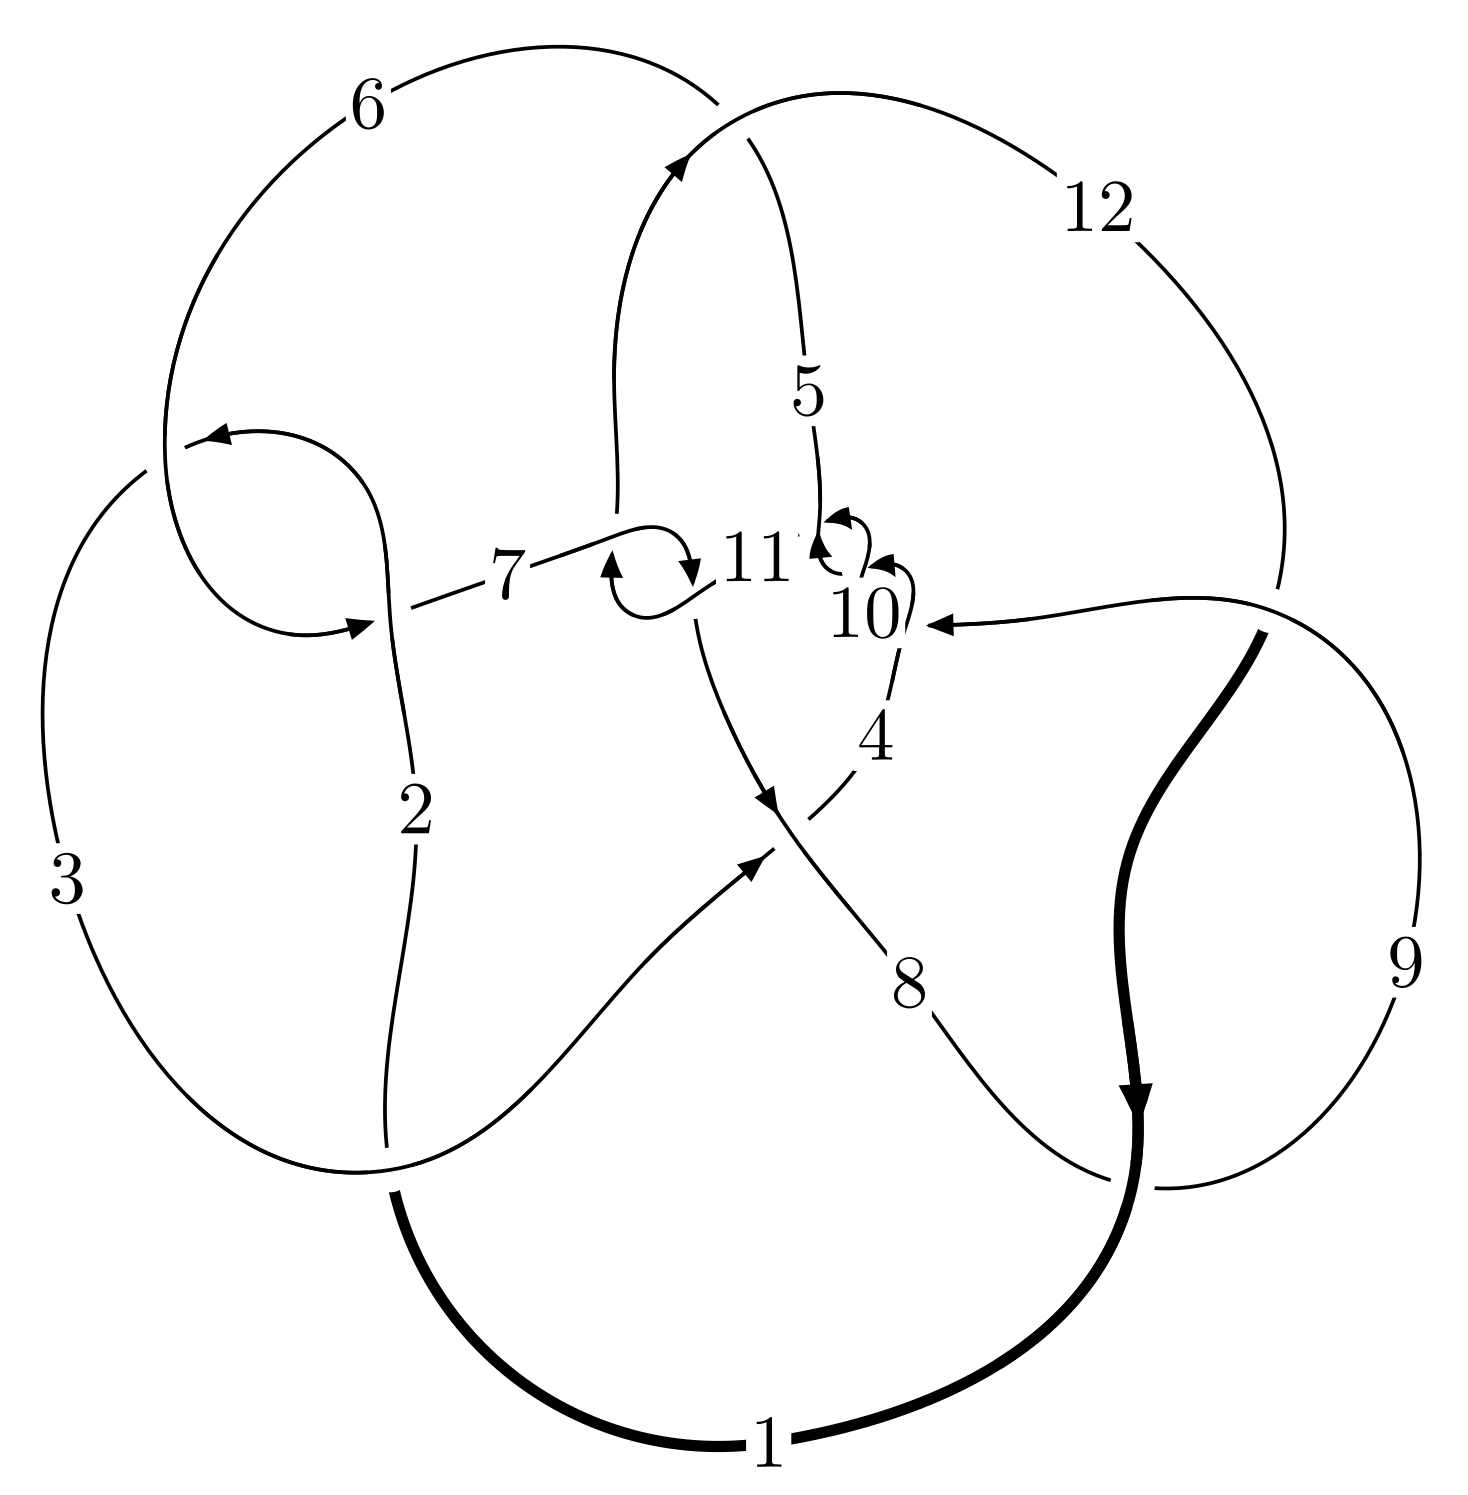
\includegraphics[width=112pt]{../../../GIT/diagram.site/Diagrams/png/1112_12a_0311.png}\\
\ \ \ A knot diagram\footnotemark}&
\allowdisplaybreaks
\textbf{Linearized knot diagam} \\
\cline{2-2}
 &
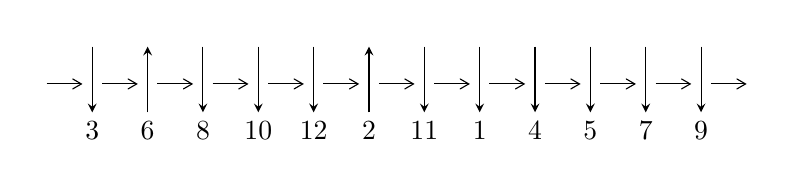
\begin{tikzpicture}[x=20pt, y=17pt]
	% nodes
	\node (C0) at (0, 0) {};
	\node (C1) at (1, 0) {};
	\node (C1U) at (1, +1) {};
	\node (C1D) at (1, -1) {3};

	\node (C2) at (2, 0) {};
	\node (C2U) at (2, +1) {};
	\node (C2D) at (2, -1) {6};

	\node (C3) at (3, 0) {};
	\node (C3U) at (3, +1) {};
	\node (C3D) at (3, -1) {8};

	\node (C4) at (4, 0) {};
	\node (C4U) at (4, +1) {};
	\node (C4D) at (4, -1) {10};

	\node (C5) at (5, 0) {};
	\node (C5U) at (5, +1) {};
	\node (C5D) at (5, -1) {12};

	\node (C6) at (6, 0) {};
	\node (C6U) at (6, +1) {};
	\node (C6D) at (6, -1) {2};

	\node (C7) at (7, 0) {};
	\node (C7U) at (7, +1) {};
	\node (C7D) at (7, -1) {11};

	\node (C8) at (8, 0) {};
	\node (C8U) at (8, +1) {};
	\node (C8D) at (8, -1) {1};

	\node (C9) at (9, 0) {};
	\node (C9U) at (9, +1) {};
	\node (C9D) at (9, -1) {4};

	\node (C10) at (10, 0) {};
	\node (C10U) at (10, +1) {};
	\node (C10D) at (10, -1) {5};

	\node (C11) at (11, 0) {};
	\node (C11U) at (11, +1) {};
	\node (C11D) at (11, -1) {7};

	\node (C12) at (12, 0) {};
	\node (C12U) at (12, +1) {};
	\node (C12D) at (12, -1) {9};
	\node (C13) at (13, 0) {};

	% arrows
	\draw[->,>={angle 60}]
	(C0) edge (C1) (C1) edge (C2) (C2) edge (C3) (C3) edge (C4) (C4) edge (C5) (C5) edge (C6) (C6) edge (C7) (C7) edge (C8) (C8) edge (C9) (C9) edge (C10) (C10) edge (C11) (C11) edge (C12) (C12) edge (C13) ;	\draw[->,>=stealth]
	(C1U) edge (C1D) (C2D) edge (C2U) (C3U) edge (C3D) (C4U) edge (C4D) (C5U) edge (C5D) (C6D) edge (C6U) (C7U) edge (C7D) (C8U) edge (C8D) (C9U) edge (C9D) (C10U) edge (C10D) (C11U) edge (C11D) (C12U) edge (C12D) ;
	\end{tikzpicture} \\
\hhline{~~} \\& 
\textbf{Solving Sequence} \\ \cline{2-2} 
 &
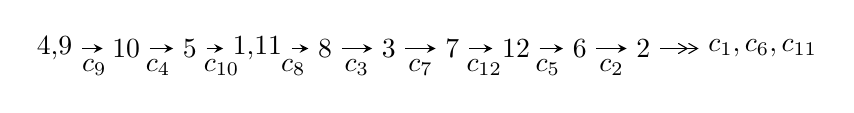
\begin{tikzpicture}[x=23pt, y=7pt]
	% node
	\node (A0) at (-1/8, 0) {4,9};
	\node (A1) at (1, 0) {10};
	\node (A2) at (2, 0) {5};
	\node (A3) at (49/16, 0) {1,11};
	\node (A4) at (33/8, 0) {8};
	\node (A5) at (41/8, 0) {3};
	\node (A6) at (49/8, 0) {7};
	\node (A7) at (57/8, 0) {12};
	\node (A8) at (65/8, 0) {6};
	\node (A9) at (73/8, 0) {2};
	\node (C1) at (1/2, -1) {$c_{9}$};
	\node (C2) at (3/2, -1) {$c_{4}$};
	\node (C3) at (5/2, -1) {$c_{10}$};
	\node (C4) at (29/8, -1) {$c_{8}$};
	\node (C5) at (37/8, -1) {$c_{3}$};
	\node (C6) at (45/8, -1) {$c_{7}$};
	\node (C7) at (53/8, -1) {$c_{12}$};
	\node (C8) at (61/8, -1) {$c_{5}$};
	\node (C9) at (69/8, -1) {$c_{2}$};
	\node (A10) at (11, 0) {$c_{1},c_{6},c_{11}$};

	% edge
	\draw[->,>=stealth]	
	(A0) edge (A1) (A1) edge (A2) (A2) edge (A3) (A3) edge (A4) (A4) edge (A5) (A5) edge (A6) (A6) edge (A7) (A7) edge (A8) (A8) edge (A9) ;
	\draw[->>,>={angle 60}]	
	(A9) edge (A10);
\end{tikzpicture} \\ 

\end{tabular} \\

\footnotetext{
The image of knot diagram is generated by the software ``\textbf{Draw programme}" developed by Andrew Bartholomew(\url{http://www.layer8.co.uk/maths/draw/index.htm\#Running-draw}), where we modified some parts for our purpose(\url{https://github.com/CATsTAILs/LinksPainter}).
}\phantom \\ \newline 
\centering \textbf{Ideals for irreducible components\footnotemark of $X_{\text{par}}$} 
 
\begin{align*}
I^u_{1}&=\langle 
4.08905\times10^{49} u^{39}-1.01301\times10^{50} u^{38}+\cdots+2.88391\times10^{51} b-2.25929\times10^{51},\\
\phantom{I^u_{1}}&\phantom{= \langle  }-4.64639\times10^{50} u^{39}+1.25973\times10^{51} u^{38}+\cdots+2.30713\times10^{52} a+9.26479\times10^{51},\\
\phantom{I^u_{1}}&\phantom{= \langle  }u^{40}-3 u^{39}+\cdots-192 u^2-32\rangle \\
I^u_{2}&=\langle 
3 u^{30} a-3 u^{30}+\cdots+5 a+11,\;-112 u^{30} a-102 u^{30}+\cdots-77 a-491,\;u^{31}+u^{30}+\cdots+2 u+1\rangle \\
I^u_{3}&=\langle 
b+1,\;8 a^2-2 a u+8 a- u+3,\;u^2-2\rangle \\
I^u_{4}&=\langle 
b+u,\;3 a-5 u+1,\;u^2+1\rangle \\
\\
I^v_{1}&=\langle 
a,\;b-1,\;4 v^2+2 v+1\rangle \\
\end{align*}
\raggedright * 5 irreducible components of $\dim_{\mathbb{C}}=0$, with total 110 representations.\\
\footnotetext{All coefficients of polynomials are rational numbers. But the coefficients are sometimes approximated in decimal forms when there is not enough margin.}
\newpage
\renewcommand{\arraystretch}{1}
\centering \section*{I. $I^u_{1}= \langle 4.09\times10^{49} u^{39}-1.01\times10^{50} u^{38}+\cdots+2.88\times10^{51} b-2.26\times10^{51},\;-4.65\times10^{50} u^{39}+1.26\times10^{51} u^{38}+\cdots+2.31\times10^{52} a+9.26\times10^{51},\;u^{40}-3 u^{39}+\cdots-192 u^2-32 \rangle$}
\flushleft \textbf{(i) Arc colorings}\\
\begin{tabular}{m{7pt} m{180pt} m{7pt} m{180pt} }
\flushright $a_{4}=$&$\begin{pmatrix}0\\u\end{pmatrix}$ \\
\flushright $a_{9}=$&$\begin{pmatrix}1\\0\end{pmatrix}$ \\
\flushright $a_{10}=$&$\begin{pmatrix}1\\u^2\end{pmatrix}$ \\
\flushright $a_{5}=$&$\begin{pmatrix}- u\\- u^3+u\end{pmatrix}$ \\
\flushright $a_{1}=$&$\begin{pmatrix}0.0201393 u^{39}-0.0546018 u^{38}+\cdots-3.01826 u-0.401572\\-0.0141788 u^{39}+0.0351264 u^{38}+\cdots+1.72761 u+0.783414\end{pmatrix}$ \\
\flushright $a_{11}=$&$\begin{pmatrix}- u^2+1\\- u^4+2 u^2\end{pmatrix}$ \\
\flushright $a_{8}=$&$\begin{pmatrix}-0.000995231 u^{39}+0.00708915 u^{38}+\cdots+0.246219 u+1.21626\\0.0112644 u^{39}-0.0355065 u^{38}+\cdots-1.56872 u-0.703111\end{pmatrix}$ \\
\flushright $a_{3}=$&$\begin{pmatrix}0.00214826 u^{39}-0.00643004 u^{38}+\cdots+1.27576 u-0.435663\\-0.00982399 u^{39}+0.0113860 u^{38}+\cdots-0.302904 u+0.425293\end{pmatrix}$ \\
\flushright $a_{7}=$&$\begin{pmatrix}0.00280373 u^{39}-0.0167005 u^{38}+\cdots-1.93511 u+0.195727\\-0.00183607 u^{39}-0.0121602 u^{38}+\cdots-0.993431 u-0.862558\end{pmatrix}$ \\
\flushright $a_{12}=$&$\begin{pmatrix}0.00596044 u^{39}-0.0194753 u^{38}+\cdots-1.29065 u+0.381841\\-0.0141788 u^{39}+0.0351264 u^{38}+\cdots+1.72761 u+0.783414\end{pmatrix}$ \\
\flushright $a_{6}=$&$\begin{pmatrix}0.00328746 u^{39}+0.00123723 u^{38}+\cdots-0.904111 u+0.0108409\\0.00995923 u^{39}-0.0198393 u^{38}+\cdots-0.266449 u+0.780010\end{pmatrix}$ \\
\flushright $a_{2}=$&$\begin{pmatrix}0.00639471 u^{39}-0.0181709 u^{38}+\cdots-0.259320 u+0.0460362\\-0.00105452 u^{39}+0.0113351 u^{38}+\cdots+0.871003 u+0.956721\end{pmatrix}$\\&\end{tabular}
\flushleft \textbf{(ii) Obstruction class $= -1$}\\~\\
\flushleft \textbf{(iii) Cusp Shapes $= 0.102467 u^{39}-0.211834 u^{38}+\cdots-12.5141 u+4.58841$}\\~\\
\newpage\renewcommand{\arraystretch}{1}
\flushleft \textbf{(iv) u-Polynomials at the component}\newline \\
\begin{tabular}{m{50pt}|m{274pt}}
Crossings & \hspace{64pt}u-Polynomials at each crossing \\
\hline $$\begin{aligned}c_{1}\end{aligned}$$&$\begin{aligned}
&u^{40}+12 u^{39}+\cdots-6305 u+64
\end{aligned}$\\
\hline $$\begin{aligned}c_{2},c_{6}\end{aligned}$$&$\begin{aligned}
&u^{40}-2 u^{39}+\cdots+57 u-8
\end{aligned}$\\
\hline $$\begin{aligned}c_{3},c_{5}\end{aligned}$$&$\begin{aligned}
&64(64 u^{40}-32 u^{39}+\cdots+40 u-8)
\end{aligned}$\\
\hline $$\begin{aligned}c_{4},c_{9},c_{10}\end{aligned}$$&$\begin{aligned}
&u^{40}+3 u^{39}+\cdots-192 u^2-32
\end{aligned}$\\
\hline $$\begin{aligned}c_{7},c_{8},c_{11}\\c_{12}\end{aligned}$$&$\begin{aligned}
&u^{40}-2 u^{39}+\cdots+19 u-7
\end{aligned}$\\
\hline
\end{tabular}\\~\\
\newpage\renewcommand{\arraystretch}{1}
\flushleft \textbf{(v) Riley Polynomials at the component}\newline \\
\begin{tabular}{m{50pt}|m{274pt}}
Crossings & \hspace{64pt}Riley Polynomials at each crossing \\
\hline $$\begin{aligned}c_{1}\end{aligned}$$&$\begin{aligned}
&y^{40}+20 y^{39}+\cdots-35596225 y+4096
\end{aligned}$\\
\hline $$\begin{aligned}c_{2},c_{6}\end{aligned}$$&$\begin{aligned}
&y^{40}+12 y^{39}+\cdots-6305 y+64
\end{aligned}$\\
\hline $$\begin{aligned}c_{3},c_{5}\end{aligned}$$&$\begin{aligned}
&4096(4096 y^{40}+3072 y^{39}+\cdots-1312 y+64)
\end{aligned}$\\
\hline $$\begin{aligned}c_{4},c_{9},c_{10}\end{aligned}$$&$\begin{aligned}
&y^{40}-35 y^{39}+\cdots+12288 y+1024
\end{aligned}$\\
\hline $$\begin{aligned}c_{7},c_{8},c_{11}\\c_{12}\end{aligned}$$&$\begin{aligned}
&y^{40}+14 y^{39}+\cdots+115 y+49
\end{aligned}$\\
\hline
\end{tabular}\\~\\
\newpage\flushleft \textbf{(vi) Complex Volumes and Cusp Shapes}
$$\begin{array}{c|c|c}  
\text{Solutions to }I^u_{1}& \I (\text{vol} + \sqrt{-1}CS) & \text{Cusp shape}\\
 \hline 
\begin{aligned}
u &= -0.440137 + 0.904158 I \\
a &= -0.46183 - 1.85321 I \\
b &= -0.513797 + 1.310640 I\end{aligned}
 & \phantom{-}6.8384 + 13.5929 I & -4.21050 - 9.23121 I \\ \hline\begin{aligned}
u &= -0.440137 - 0.904158 I \\
a &= -0.46183 + 1.85321 I \\
b &= -0.513797 - 1.310640 I\end{aligned}
 & \phantom{-}6.8384 - 13.5929 I & -4.21050 + 9.23121 I \\ \hline\begin{aligned}
u &= \phantom{-}0.429948 + 0.950952 I \\
a &= -0.40500 + 1.76947 I \\
b &= -0.420528 - 1.284740 I\end{aligned}
 & \phantom{-}8.33666 - 7.25783 I & -2.07869 + 5.28616 I \\ \hline\begin{aligned}
u &= \phantom{-}0.429948 - 0.950952 I \\
a &= -0.40500 - 1.76947 I \\
b &= -0.420528 + 1.284740 I\end{aligned}
 & \phantom{-}8.33666 + 7.25783 I & -2.07869 - 5.28616 I \\ \hline\begin{aligned}
u &= -0.187511 + 0.912417 I \\
a &= \phantom{-}0.02873 - 1.86648 I \\
b &= -0.409629 + 0.962631 I\end{aligned}
 & -0.05063 + 5.82607 I & -8.03423 - 8.68283 I \\ \hline\begin{aligned}
u &= -0.187511 - 0.912417 I \\
a &= \phantom{-}0.02873 + 1.86648 I \\
b &= -0.409629 - 0.962631 I\end{aligned}
 & -0.05063 - 5.82607 I & -8.03423 + 8.68283 I \\ \hline\begin{aligned}
u &= -0.808683 + 0.827619 I \\
a &= -0.582063 - 1.047810 I \\
b &= \phantom{-}0.378612 + 1.207320 I\end{aligned}
 & \phantom{-}5.82044 - 7.81253 I & -4.24739 + 6.17178 I \\ \hline\begin{aligned}
u &= -0.808683 - 0.827619 I \\
a &= -0.582063 + 1.047810 I \\
b &= \phantom{-}0.378612 - 1.207320 I\end{aligned}
 & \phantom{-}5.82044 + 7.81253 I & -4.24739 - 6.17178 I \\ \hline\begin{aligned}
u &= \phantom{-}1.199590 + 0.427748 I \\
a &= \phantom{-}0.411698 - 1.287580 I \\
b &= \phantom{-}0.387145 + 0.855456 I\end{aligned}
 & -3.26360 - 1.49706 I & -11.41293 + 5.34755 I \\ \hline\begin{aligned}
u &= \phantom{-}1.199590 - 0.427748 I \\
a &= \phantom{-}0.411698 + 1.287580 I \\
b &= \phantom{-}0.387145 - 0.855456 I\end{aligned}
 & -3.26360 + 1.49706 I & -11.41293 - 5.34755 I\\
 \hline 
 \end{array}$$\newpage$$\begin{array}{c|c|c}  
\text{Solutions to }I^u_{1}& \I (\text{vol} + \sqrt{-1}CS) & \text{Cusp shape}\\
 \hline 
\begin{aligned}
u &= \phantom{-}0.907718 + 0.908783 I \\
a &= -0.490822 + 1.072100 I \\
b &= \phantom{-}0.255927 - 1.148880 I\end{aligned}
 & \phantom{-}7.10406 + 1.09362 I & -1.87527 - 4.00746 I \\ \hline\begin{aligned}
u &= \phantom{-}0.907718 - 0.908783 I \\
a &= -0.490822 - 1.072100 I \\
b &= \phantom{-}0.255927 + 1.148880 I\end{aligned}
 & \phantom{-}7.10406 - 1.09362 I & -1.87527 + 4.00746 I \\ \hline\begin{aligned}
u &= -0.227717 + 1.277080 I \\
a &= \phantom{-}0.170112 + 1.366760 I \\
b &= -0.110689 - 0.909064 I\end{aligned}
 & \phantom{-}4.51263 - 0.64388 I & -12.6147 + 10.6040 I \\ \hline\begin{aligned}
u &= -0.227717 - 1.277080 I \\
a &= \phantom{-}0.170112 - 1.366760 I \\
b &= -0.110689 + 0.909064 I\end{aligned}
 & \phantom{-}4.51263 + 0.64388 I & -12.6147 - 10.6040 I \\ \hline\begin{aligned}
u &= -1.337180 + 0.093481 I \\
a &= -0.568363 - 0.175872 I \\
b &= -1.40862 - 0.31480 I\end{aligned}
 & -5.44648 - 0.82010 I & -6.94084 - 0.88214 I \\ \hline\begin{aligned}
u &= -1.337180 - 0.093481 I \\
a &= -0.568363 + 0.175872 I \\
b &= -1.40862 + 0.31480 I\end{aligned}
 & -5.44648 + 0.82010 I & -6.94084 + 0.88214 I \\ \hline\begin{aligned}
u &= \phantom{-}1.363060 + 0.137405 I \\
a &= -0.477079 + 0.243693 I \\
b &= -1.40170 + 0.49884 I\end{aligned}
 & -6.07938 - 4.11851 I & -9.52490 + 6.62129 I \\ \hline\begin{aligned}
u &= \phantom{-}1.363060 - 0.137405 I \\
a &= -0.477079 - 0.243693 I \\
b &= -1.40170 - 0.49884 I\end{aligned}
 & -6.07938 + 4.11851 I & -9.52490 - 6.62129 I \\ \hline\begin{aligned}
u &= -0.527569 + 0.240579 I \\
a &= -0.374770 - 0.519466 I \\
b &= \phantom{-}0.732459 + 0.494483 I\end{aligned}
 & -2.68524 - 2.28522 I & -15.8983 + 1.9193 I \\ \hline\begin{aligned}
u &= -0.527569 - 0.240579 I \\
a &= -0.374770 + 0.519466 I \\
b &= \phantom{-}0.732459 - 0.494483 I\end{aligned}
 & -2.68524 + 2.28522 I & -15.8983 - 1.9193 I\\
 \hline 
 \end{array}$$\newpage$$\begin{array}{c|c|c}  
\text{Solutions to }I^u_{1}& \I (\text{vol} + \sqrt{-1}CS) & \text{Cusp shape}\\
 \hline 
\begin{aligned}
u &= -1.43224\phantom{ +0.000000I} \\
a &= -0.492239\phantom{ +0.000000I} \\
b &= -0.887681\phantom{ +0.000000I}\end{aligned}
 & -6.54259\phantom{ +0.000000I} & -14.4120\phantom{ +0.000000I} \\ \hline\begin{aligned}
u &= \phantom{-}1.47203 + 0.11321 I \\
a &= -0.308809 + 0.057755 I \\
b &= -0.961493 + 0.650737 I\end{aligned}
 & -9.12443 + 0.78989 I & -16.6960 - 1.5011 I \\ \hline\begin{aligned}
u &= \phantom{-}1.47203 - 0.11321 I \\
a &= -0.308809 - 0.057755 I \\
b &= -0.961493 - 0.650737 I\end{aligned}
 & -9.12443 - 0.78989 I & -16.6960 + 1.5011 I \\ \hline\begin{aligned}
u &= \phantom{-}1.44029 + 0.35968 I \\
a &= \phantom{-}0.89871 - 1.21509 I \\
b &= \phantom{-}0.577709 + 1.136010 I\end{aligned}
 & -5.34996 - 10.39560 I & -11.35294 + 7.92882 I \\ \hline\begin{aligned}
u &= \phantom{-}1.44029 - 0.35968 I \\
a &= \phantom{-}0.89871 + 1.21509 I \\
b &= \phantom{-}0.577709 - 1.136010 I\end{aligned}
 & -5.34996 + 10.39560 I & -11.35294 - 7.92882 I \\ \hline\begin{aligned}
u &= -1.42057 + 0.48007 I \\
a &= \phantom{-}0.631676 + 1.097510 I \\
b &= \phantom{-}0.374302 - 1.088160 I\end{aligned}
 & \phantom{-}0.17053 + 6.80496 I & -8.00000 - 8.25092 I \\ \hline\begin{aligned}
u &= -1.42057 - 0.48007 I \\
a &= \phantom{-}0.631676 - 1.097510 I \\
b &= \phantom{-}0.374302 + 1.088160 I\end{aligned}
 & \phantom{-}0.17053 - 6.80496 I & -8.00000 + 8.25092 I \\ \hline\begin{aligned}
u &= -1.51413 + 0.15368 I \\
a &= -0.505558 - 0.545335 I \\
b &= -0.073480 + 0.597284 I\end{aligned}
 & -4.25095 - 1.64346 I & -8.00000 + 0. I\phantom{ +0.000000I} \\ \hline\begin{aligned}
u &= -1.51413 - 0.15368 I \\
a &= -0.505558 + 0.545335 I \\
b &= -0.073480 - 0.597284 I\end{aligned}
 & -4.25095 + 1.64346 I & -8.00000 + 0. I\phantom{ +0.000000I} \\ \hline\begin{aligned}
u &= \phantom{-}1.50913 + 0.33966 I \\
a &= \phantom{-}1.10053 - 1.00347 I \\
b &= \phantom{-}0.63668 + 1.33597 I\end{aligned}
 & \phantom{-}0.5699 - 18.1001 I & \phantom{-0.000000 -}0. + 9.77509 I\\
 \hline 
 \end{array}$$\newpage$$\begin{array}{c|c|c}  
\text{Solutions to }I^u_{1}& \I (\text{vol} + \sqrt{-1}CS) & \text{Cusp shape}\\
 \hline 
\begin{aligned}
u &= \phantom{-}1.50913 - 0.33966 I \\
a &= \phantom{-}1.10053 + 1.00347 I \\
b &= \phantom{-}0.63668 - 1.33597 I\end{aligned}
 & \phantom{-}0.5699 + 18.1001 I & \phantom{-0.000000 } 0. - 9.77509 I \\ \hline\begin{aligned}
u &= -1.50745 + 0.35840 I \\
a &= \phantom{-}1.01596 + 0.98674 I \\
b &= \phantom{-}0.57197 - 1.32042 I\end{aligned}
 & \phantom{-}2.12914 + 11.97580 I & \phantom{-0.000000 } 0 \\ \hline\begin{aligned}
u &= -1.50745 - 0.35840 I \\
a &= \phantom{-}1.01596 - 0.98674 I \\
b &= \phantom{-}0.57197 + 1.32042 I\end{aligned}
 & \phantom{-}2.12914 - 11.97580 I & \phantom{-0.000000 } 0 \\ \hline\begin{aligned}
u &= \phantom{-}0.398385\phantom{ +0.000000I} \\
a &= \phantom{-}0.194086\phantom{ +0.000000I} \\
b &= \phantom{-}0.411087\phantom{ +0.000000I}\end{aligned}
 & -0.650198\phantom{ +0.000000I} & -15.0380\phantom{ +0.000000I} \\ \hline\begin{aligned}
u &= \phantom{-}0.060206 + 0.390625 I \\
a &= \phantom{-}1.81385 - 0.89243 I \\
b &= -0.311880 + 0.206339 I\end{aligned}
 & -0.52443 - 1.67679 I & -4.14197 + 2.11677 I \\ \hline\begin{aligned}
u &= \phantom{-}0.060206 - 0.390625 I \\
a &= \phantom{-}1.81385 + 0.89243 I \\
b &= -0.311880 - 0.206339 I\end{aligned}
 & -0.52443 + 1.67679 I & -4.14197 - 2.11677 I \\ \hline\begin{aligned}
u &= -0.085016 + 0.355683 I \\
a &= -0.687889 - 0.084642 I \\
b &= \phantom{-}1.230980 + 0.116031 I\end{aligned}
 & -1.36201 + 2.26426 I & \phantom{-}3.25236 - 9.63689 I \\ \hline\begin{aligned}
u &= -0.085016 - 0.355683 I \\
a &= -0.687889 + 0.084642 I \\
b &= \phantom{-}1.230980 - 0.116031 I\end{aligned}
 & -1.36201 - 2.26426 I & \phantom{-}3.25236 + 9.63689 I \\ \hline\begin{aligned}
u &= \phantom{-}1.69092 + 0.00044 I \\
a &= -0.185011 + 0.410776 I \\
b &= -0.295674 - 0.847006 I\end{aligned}
 & -3.61784 - 4.35903 I & \phantom{-0.000000 } 0 \\ \hline\begin{aligned}
u &= \phantom{-}1.69092 - 0.00044 I \\
a &= -0.185011 - 0.410776 I \\
b &= -0.295674 + 0.847006 I\end{aligned}
 & -3.61784 + 4.35903 I & \phantom{-0.000000 } 0\\
 \hline 
 \end{array}$$\newpage\newpage\renewcommand{\arraystretch}{1}
\centering \section*{II. $I^u_{2}= \langle 3 u^{30} a-3 u^{30}+\cdots+5 a+11,\;-112 u^{30} a-102 u^{30}+\cdots-77 a-491,\;u^{31}+u^{30}+\cdots+2 u+1 \rangle$}
\flushleft \textbf{(i) Arc colorings}\\
\begin{tabular}{m{7pt} m{180pt} m{7pt} m{180pt} }
\flushright $a_{4}=$&$\begin{pmatrix}0\\u\end{pmatrix}$ \\
\flushright $a_{9}=$&$\begin{pmatrix}1\\0\end{pmatrix}$ \\
\flushright $a_{10}=$&$\begin{pmatrix}1\\u^2\end{pmatrix}$ \\
\flushright $a_{5}=$&$\begin{pmatrix}- u\\- u^3+u\end{pmatrix}$ \\
\flushright $a_{1}=$&$\begin{pmatrix}a\\-0.187500 a u^{30}+0.187500 u^{30}+\cdots-0.312500 a-0.687500\end{pmatrix}$ \\
\flushright $a_{11}=$&$\begin{pmatrix}- u^2+1\\- u^4+2 u^2\end{pmatrix}$ \\
\flushright $a_{8}=$&$\begin{pmatrix}0.187500 a u^{30}+1.52679 u^{30}+\cdots-0.687500 a+2.11607\\0.187500 a u^{30}-0.187500 u^{30}+\cdots+0.312500 a+0.687500\end{pmatrix}$ \\
\flushright $a_{3}=$&$\begin{pmatrix}0.830357 a u^{30}-1.21811 u^{30}+\cdots+2.09821 a+0.554847\\-0.625000 a u^{30}-0.232143 u^{30}+\cdots-0.375000 a-1.33929\end{pmatrix}$ \\
\flushright $a_{7}=$&$\begin{pmatrix}0.187500 a u^{30}+1.52679 u^{30}+\cdots-0.687500 a+1.11607\\1\end{pmatrix}$ \\
\flushright $a_{12}=$&$\begin{pmatrix}-0.187500 a u^{30}+0.187500 u^{30}+\cdots+0.687500 a-0.687500\\-0.187500 a u^{30}+0.187500 u^{30}+\cdots-0.312500 a-0.687500\end{pmatrix}$ \\
\flushright $a_{6}=$&$\begin{pmatrix}0.232143 a u^{30}-2.41582 u^{30}+\cdots+1.33929 a-1.13520\\-0.312500 a u^{30}-0.830357 u^{30}+\cdots-0.187500 a-2.09821\end{pmatrix}$ \\
\flushright $a_{2}=$&$\begin{pmatrix}-0.758929 a u^{30}-0.547194 u^{30}+\cdots+1.54464 a-1.87117\\-0.562500 a u^{30}-0.00892857 u^{30}+\cdots-0.937500 a-1.20536\end{pmatrix}$\\&\end{tabular}
\flushleft \textbf{(ii) Obstruction class $= -1$}\\~\\
\flushleft \textbf{(iii) Cusp Shapes $= 4 u^{28}-52 u^{26}+4 u^{25}+292 u^{24}-48 u^{23}-916 u^{22}+244 u^{21}+1732 u^{20}-672 u^{19}-1988 u^{18}+1056 u^{17}+1360 u^{16}-896 u^{15}-644 u^{14}+332 u^{13}+420 u^{12}-60 u^{11}-288 u^{10}+84 u^9+88 u^8-16 u^6-44 u^5+4 u^2-16 u-10$}\\~\\
\newpage\renewcommand{\arraystretch}{1}
\flushleft \textbf{(iv) u-Polynomials at the component}\newline \\
\begin{tabular}{m{50pt}|m{274pt}}
Crossings & \hspace{64pt}u-Polynomials at each crossing \\
\hline $$\begin{aligned}c_{1}\end{aligned}$$&$\begin{aligned}
&(u^{31}+11 u^{30}+\cdots-4 u-1)^{2}
\end{aligned}$\\
\hline $$\begin{aligned}c_{2},c_{6}\end{aligned}$$&$\begin{aligned}
&(u^{31}- u^{30}+\cdots+2 u^2+1)^{2}
\end{aligned}$\\
\hline $$\begin{aligned}c_{3},c_{5}\end{aligned}$$&$\begin{aligned}
&49(49 u^{62}-259 u^{61}+\cdots-1.07072\times10^{7} u+1308800)
\end{aligned}$\\
\hline $$\begin{aligned}c_{4},c_{9},c_{10}\end{aligned}$$&$\begin{aligned}
&(u^{31}- u^{30}+\cdots+2 u-1)^{2}
\end{aligned}$\\
\hline $$\begin{aligned}c_{7},c_{8},c_{11}\\c_{12}\end{aligned}$$&$\begin{aligned}
&u^{62}+5 u^{61}+\cdots+101 u+10
\end{aligned}$\\
\hline
\end{tabular}\\~\\
\newpage\renewcommand{\arraystretch}{1}
\flushleft \textbf{(v) Riley Polynomials at the component}\newline \\
\begin{tabular}{m{50pt}|m{274pt}}
Crossings & \hspace{64pt}Riley Polynomials at each crossing \\
\hline $$\begin{aligned}c_{1}\end{aligned}$$&$\begin{aligned}
&(y^{31}+19 y^{30}+\cdots-8 y-1)^{2}
\end{aligned}$\\
\hline $$\begin{aligned}c_{2},c_{6}\end{aligned}$$&$\begin{aligned}
&(y^{31}+11 y^{30}+\cdots-4 y-1)^{2}
\end{aligned}$\\
\hline $$\begin{aligned}c_{3},c_{5}\end{aligned}$$&$\begin{aligned}
&2401\\
&\cdot(2401 y^{62}+64827 y^{61}+\cdots-13911596441600 y+1712957440000)
\end{aligned}$\\
\hline $$\begin{aligned}c_{4},c_{9},c_{10}\end{aligned}$$&$\begin{aligned}
&(y^{31}-29 y^{30}+\cdots-4 y-1)^{2}
\end{aligned}$\\
\hline $$\begin{aligned}c_{7},c_{8},c_{11}\\c_{12}\end{aligned}$$&$\begin{aligned}
&y^{62}+39 y^{61}+\cdots+1299 y+100
\end{aligned}$\\
\hline
\end{tabular}\\~\\
\newpage\flushleft \textbf{(vi) Complex Volumes and Cusp Shapes}
$$\begin{array}{c|c|c}  
\text{Solutions to }I^u_{2}& \I (\text{vol} + \sqrt{-1}CS) & \text{Cusp shape}\\
 \hline 
\begin{aligned}
u &= -1.196790 + 0.189244 I \\
a &= \phantom{-}1.281310 + 0.314655 I \\
b &= \phantom{-}0.736083 - 1.151530 I\end{aligned}
 & \phantom{-}3.79282 + 0.40298 I & -4.92930 - 0.52831 I \\ \hline\begin{aligned}
u &= -1.196790 + 0.189244 I \\
a &= \phantom{-}0.029998 - 0.447048 I \\
b &= \phantom{-}0.31189 + 1.51073 I\end{aligned}
 & \phantom{-}3.79282 + 0.40298 I & -4.92930 - 0.52831 I \\ \hline\begin{aligned}
u &= -1.196790 - 0.189244 I \\
a &= \phantom{-}1.281310 - 0.314655 I \\
b &= \phantom{-}0.736083 + 1.151530 I\end{aligned}
 & \phantom{-}3.79282 - 0.40298 I & -4.92930 + 0.52831 I \\ \hline\begin{aligned}
u &= -1.196790 - 0.189244 I \\
a &= \phantom{-}0.029998 + 0.447048 I \\
b &= \phantom{-}0.31189 - 1.51073 I\end{aligned}
 & \phantom{-}3.79282 - 0.40298 I & -4.92930 + 0.52831 I \\ \hline\begin{aligned}
u &= \phantom{-}0.371332 + 0.681959 I \\
a &= \phantom{-}0.437240 + 0.099266 I \\
b &= -1.025610 + 0.013746 I\end{aligned}
 & \phantom{-}2.81425 - 8.17190 I & -6.44268 + 8.00325 I \\ \hline\begin{aligned}
u &= \phantom{-}0.371332 + 0.681959 I \\
a &= \phantom{-}0.40027 - 1.90954 I \\
b &= \phantom{-}0.52071 + 1.33060 I\end{aligned}
 & \phantom{-}2.81425 - 8.17190 I & -6.44268 + 8.00325 I \\ \hline\begin{aligned}
u &= \phantom{-}0.371332 - 0.681959 I \\
a &= \phantom{-}0.437240 - 0.099266 I \\
b &= -1.025610 - 0.013746 I\end{aligned}
 & \phantom{-}2.81425 + 8.17190 I & -6.44268 - 8.00325 I \\ \hline\begin{aligned}
u &= \phantom{-}0.371332 - 0.681959 I \\
a &= \phantom{-}0.40027 + 1.90954 I \\
b &= \phantom{-}0.52071 - 1.33060 I\end{aligned}
 & \phantom{-}2.81425 + 8.17190 I & -6.44268 - 8.00325 I \\ \hline\begin{aligned}
u &= \phantom{-}0.434998 + 0.611250 I \\
a &= \phantom{-}0.553711 - 0.502128 I \\
b &= -0.543967 + 0.395556 I\end{aligned}
 & -1.60703 - 1.99617 I & -11.89924 + 3.62729 I \\ \hline\begin{aligned}
u &= \phantom{-}0.434998 + 0.611250 I \\
a &= \phantom{-}0.48079 - 1.60306 I \\
b &= \phantom{-}0.423951 + 0.864140 I\end{aligned}
 & -1.60703 - 1.99617 I & -11.89924 + 3.62729 I\\
 \hline 
 \end{array}$$\newpage$$\begin{array}{c|c|c}  
\text{Solutions to }I^u_{2}& \I (\text{vol} + \sqrt{-1}CS) & \text{Cusp shape}\\
 \hline 
\begin{aligned}
u &= \phantom{-}0.434998 - 0.611250 I \\
a &= \phantom{-}0.553711 + 0.502128 I \\
b &= -0.543967 - 0.395556 I\end{aligned}
 & -1.60703 + 1.99617 I & -11.89924 - 3.62729 I \\ \hline\begin{aligned}
u &= \phantom{-}0.434998 - 0.611250 I \\
a &= \phantom{-}0.48079 + 1.60306 I \\
b &= \phantom{-}0.423951 - 0.864140 I\end{aligned}
 & -1.60703 + 1.99617 I & -11.89924 - 3.62729 I \\ \hline\begin{aligned}
u &= \phantom{-}1.239060 + 0.217665 I \\
a &= \phantom{-}1.244900 - 0.296015 I \\
b &= \phantom{-}0.843023 + 1.049800 I\end{aligned}
 & \phantom{-}3.41810 - 5.89464 I & -5.94513 + 6.44091 I \\ \hline\begin{aligned}
u &= \phantom{-}1.239060 + 0.217665 I \\
a &= -0.213070 + 0.516323 I \\
b &= \phantom{-}0.20988 - 1.57615 I\end{aligned}
 & \phantom{-}3.41810 - 5.89464 I & -5.94513 + 6.44091 I \\ \hline\begin{aligned}
u &= \phantom{-}1.239060 - 0.217665 I \\
a &= \phantom{-}1.244900 + 0.296015 I \\
b &= \phantom{-}0.843023 - 1.049800 I\end{aligned}
 & \phantom{-}3.41810 + 5.89464 I & -5.94513 - 6.44091 I \\ \hline\begin{aligned}
u &= \phantom{-}1.239060 - 0.217665 I \\
a &= -0.213070 - 0.516323 I \\
b &= \phantom{-}0.20988 + 1.57615 I\end{aligned}
 & \phantom{-}3.41810 + 5.89464 I & -5.94513 - 6.44091 I \\ \hline\begin{aligned}
u &= \phantom{-}0.529247 + 0.517876 I \\
a &= \phantom{-}0.053894 - 1.405920 I \\
b &= \phantom{-}0.588857 - 0.075465 I\end{aligned}
 & \phantom{-}2.14842 + 4.14236 I & -8.20039 - 2.04013 I \\ \hline\begin{aligned}
u &= \phantom{-}0.529247 + 0.517876 I \\
a &= \phantom{-}1.44126 - 0.83676 I \\
b &= -0.264698 + 1.158750 I\end{aligned}
 & \phantom{-}2.14842 + 4.14236 I & -8.20039 - 2.04013 I \\ \hline\begin{aligned}
u &= \phantom{-}0.529247 - 0.517876 I \\
a &= \phantom{-}0.053894 + 1.405920 I \\
b &= \phantom{-}0.588857 + 0.075465 I\end{aligned}
 & \phantom{-}2.14842 - 4.14236 I & -8.20039 + 2.04013 I \\ \hline\begin{aligned}
u &= \phantom{-}0.529247 - 0.517876 I \\
a &= \phantom{-}1.44126 + 0.83676 I \\
b &= -0.264698 - 1.158750 I\end{aligned}
 & \phantom{-}2.14842 - 4.14236 I & -8.20039 + 2.04013 I\\
 \hline 
 \end{array}$$\newpage$$\begin{array}{c|c|c}  
\text{Solutions to }I^u_{2}& \I (\text{vol} + \sqrt{-1}CS) & \text{Cusp shape}\\
 \hline 
\begin{aligned}
u &= -0.343506 + 0.654959 I \\
a &= \phantom{-}0.213125 - 0.091385 I \\
b &= -0.878890 + 0.145845 I\end{aligned}
 & \phantom{-}4.01963 + 2.73446 I & -4.23310 - 3.38925 I \\ \hline\begin{aligned}
u &= -0.343506 + 0.654959 I \\
a &= \phantom{-}0.47531 + 1.96420 I \\
b &= \phantom{-}0.362702 - 1.325630 I\end{aligned}
 & \phantom{-}4.01963 + 2.73446 I & -4.23310 - 3.38925 I \\ \hline\begin{aligned}
u &= -0.343506 - 0.654959 I \\
a &= \phantom{-}0.213125 + 0.091385 I \\
b &= -0.878890 - 0.145845 I\end{aligned}
 & \phantom{-}4.01963 - 2.73446 I & -4.23310 + 3.38925 I \\ \hline\begin{aligned}
u &= -0.343506 - 0.654959 I \\
a &= \phantom{-}0.47531 - 1.96420 I \\
b &= \phantom{-}0.362702 + 1.325630 I\end{aligned}
 & \phantom{-}4.01963 - 2.73446 I & -4.23310 + 3.38925 I \\ \hline\begin{aligned}
u &= -1.26234\phantom{ +0.000000I} \\
a &= \phantom{-}1.24705 + 1.05057 I \\
b &= \phantom{-}0.323876 - 1.146600 I\end{aligned}
 & \phantom{-}0.537061\phantom{ +0.000000I} & -5.58210\phantom{ +0.000000I} \\ \hline\begin{aligned}
u &= -1.26234\phantom{ +0.000000I} \\
a &= \phantom{-}1.24705 - 1.05057 I \\
b &= \phantom{-}0.323876 + 1.146600 I\end{aligned}
 & \phantom{-}0.537061\phantom{ +0.000000I} & -5.58210\phantom{ +0.000000I} \\ \hline\begin{aligned}
u &= -0.028009 + 0.652167 I \\
a &= -0.30680 - 1.72943 I \\
b &= -0.573998 + 1.285130 I\end{aligned}
 & \phantom{-}7.28578 + 2.71284 I & -0.10058 - 3.44665 I \\ \hline\begin{aligned}
u &= -0.028009 + 0.652167 I \\
a &= -0.19450 + 1.96096 I \\
b &= -0.45397 - 1.38921 I\end{aligned}
 & \phantom{-}7.28578 + 2.71284 I & -0.10058 - 3.44665 I \\ \hline\begin{aligned}
u &= -0.028009 - 0.652167 I \\
a &= -0.30680 + 1.72943 I \\
b &= -0.573998 - 1.285130 I\end{aligned}
 & \phantom{-}7.28578 - 2.71284 I & -0.10058 + 3.44665 I \\ \hline\begin{aligned}
u &= -0.028009 - 0.652167 I \\
a &= -0.19450 - 1.96096 I \\
b &= -0.45397 + 1.38921 I\end{aligned}
 & \phantom{-}7.28578 - 2.71284 I & -0.10058 + 3.44665 I\\
 \hline 
 \end{array}$$\newpage$$\begin{array}{c|c|c}  
\text{Solutions to }I^u_{2}& \I (\text{vol} + \sqrt{-1}CS) & \text{Cusp shape}\\
 \hline 
\begin{aligned}
u &= \phantom{-}1.358560 + 0.080822 I \\
a &= -0.49901 + 2.29998 I \\
b &= \phantom{-}0.076735 - 1.182270 I\end{aligned}
 & -1.93424 - 2.56488 I & -13.16453 + 4.43258 I \\ \hline\begin{aligned}
u &= \phantom{-}1.358560 + 0.080822 I \\
a &= \phantom{-}2.36676 + 0.38002 I \\
b &= \phantom{-}0.267326 + 0.813715 I\end{aligned}
 & -1.93424 - 2.56488 I & -13.16453 + 4.43258 I \\ \hline\begin{aligned}
u &= \phantom{-}1.358560 - 0.080822 I \\
a &= -0.49901 - 2.29998 I \\
b &= \phantom{-}0.076735 + 1.182270 I\end{aligned}
 & -1.93424 + 2.56488 I & -13.16453 - 4.43258 I \\ \hline\begin{aligned}
u &= \phantom{-}1.358560 - 0.080822 I \\
a &= \phantom{-}2.36676 - 0.38002 I \\
b &= \phantom{-}0.267326 - 0.813715 I\end{aligned}
 & -1.93424 + 2.56488 I & -13.16453 - 4.43258 I \\ \hline\begin{aligned}
u &= -0.464772 + 0.428483 I \\
a &= -0.21337 + 1.49668 I \\
b &= \phantom{-}0.274726 + 0.400923 I\end{aligned}
 & \phantom{-}3.29780 + 0.92992 I & -6.40372 - 3.68841 I \\ \hline\begin{aligned}
u &= -0.464772 + 0.428483 I \\
a &= \phantom{-}1.87218 + 1.29697 I \\
b &= -0.052308 - 1.171690 I\end{aligned}
 & \phantom{-}3.29780 + 0.92992 I & -6.40372 - 3.68841 I \\ \hline\begin{aligned}
u &= -0.464772 - 0.428483 I \\
a &= -0.21337 - 1.49668 I \\
b &= \phantom{-}0.274726 - 0.400923 I\end{aligned}
 & \phantom{-}3.29780 - 0.92992 I & -6.40372 + 3.68841 I \\ \hline\begin{aligned}
u &= -0.464772 - 0.428483 I \\
a &= \phantom{-}1.87218 - 1.29697 I \\
b &= -0.052308 + 1.171690 I\end{aligned}
 & \phantom{-}3.29780 - 0.92992 I & -6.40372 + 3.68841 I \\ \hline\begin{aligned}
u &= \phantom{-}1.43568 + 0.18978 I \\
a &= -0.939070 + 0.829544 I \\
b &= -0.275288 - 1.076150 I\end{aligned}
 & -2.60250 - 3.33239 I & -9.23670 + 3.21859 I \\ \hline\begin{aligned}
u &= \phantom{-}1.43568 + 0.18978 I \\
a &= \phantom{-}0.289833 + 0.332892 I \\
b &= \phantom{-}0.521278 - 0.041093 I\end{aligned}
 & -2.60250 - 3.33239 I & -9.23670 + 3.21859 I\\
 \hline 
 \end{array}$$\newpage$$\begin{array}{c|c|c}  
\text{Solutions to }I^u_{2}& \I (\text{vol} + \sqrt{-1}CS) & \text{Cusp shape}\\
 \hline 
\begin{aligned}
u &= \phantom{-}1.43568 - 0.18978 I \\
a &= -0.939070 - 0.829544 I \\
b &= -0.275288 + 1.076150 I\end{aligned}
 & -2.60250 + 3.33239 I & -9.23670 - 3.21859 I \\ \hline\begin{aligned}
u &= \phantom{-}1.43568 - 0.18978 I \\
a &= \phantom{-}0.289833 - 0.332892 I \\
b &= \phantom{-}0.521278 + 0.041093 I\end{aligned}
 & -2.60250 + 3.33239 I & -9.23670 - 3.21859 I \\ \hline\begin{aligned}
u &= \phantom{-}1.43808 + 0.24908 I \\
a &= -0.968905 + 0.795580 I \\
b &= -0.61976 - 1.34317 I\end{aligned}
 & -1.70250 - 6.04082 I & -8.35365 + 3.16093 I \\ \hline\begin{aligned}
u &= \phantom{-}1.43808 + 0.24908 I \\
a &= \phantom{-}0.393198 - 0.274074 I \\
b &= \phantom{-}1.120860 - 0.098271 I\end{aligned}
 & -1.70250 - 6.04082 I & -8.35365 + 3.16093 I \\ \hline\begin{aligned}
u &= \phantom{-}1.43808 - 0.24908 I \\
a &= -0.968905 - 0.795580 I \\
b &= -0.61976 + 1.34317 I\end{aligned}
 & -1.70250 + 6.04082 I & -8.35365 - 3.16093 I \\ \hline\begin{aligned}
u &= \phantom{-}1.43808 - 0.24908 I \\
a &= \phantom{-}0.393198 + 0.274074 I \\
b &= \phantom{-}1.120860 + 0.098271 I\end{aligned}
 & -1.70250 + 6.04082 I & -8.35365 - 3.16093 I \\ \hline\begin{aligned}
u &= -1.45066 + 0.25754 I \\
a &= -1.008450 - 0.802446 I \\
b &= -0.73854 + 1.34705 I\end{aligned}
 & -3.04348 + 11.60290 I & -10.34947 - 7.70694 I \\ \hline\begin{aligned}
u &= -1.45066 + 0.25754 I \\
a &= \phantom{-}0.334822 + 0.373412 I \\
b &= \phantom{-}1.219230 + 0.204321 I\end{aligned}
 & -3.04348 + 11.60290 I & -10.34947 - 7.70694 I \\ \hline\begin{aligned}
u &= -1.45066 - 0.25754 I \\
a &= -1.008450 + 0.802446 I \\
b &= -0.73854 - 1.34705 I\end{aligned}
 & -3.04348 - 11.60290 I & -10.34947 + 7.70694 I \\ \hline\begin{aligned}
u &= -1.45066 - 0.25754 I \\
a &= \phantom{-}0.334822 - 0.373412 I \\
b &= \phantom{-}1.219230 - 0.204321 I\end{aligned}
 & -3.04348 - 11.60290 I & -10.34947 + 7.70694 I\\
 \hline 
 \end{array}$$\newpage$$\begin{array}{c|c|c}  
\text{Solutions to }I^u_{2}& \I (\text{vol} + \sqrt{-1}CS) & \text{Cusp shape}\\
 \hline 
\begin{aligned}
u &= -1.46473 + 0.17711 I \\
a &= -0.752786 - 0.694476 I \\
b &= -0.144612 + 0.731261 I\end{aligned}
 & -4.22211 - 1.64856 I & -12.01509 + 2.12263 I \\ \hline\begin{aligned}
u &= -1.46473 + 0.17711 I \\
a &= -0.319336 - 0.515774 I \\
b &= \phantom{-}0.172653 + 0.424747 I\end{aligned}
 & -4.22211 - 1.64856 I & -12.01509 + 2.12263 I \\ \hline\begin{aligned}
u &= -1.46473 - 0.17711 I \\
a &= -0.752786 + 0.694476 I \\
b &= -0.144612 - 0.731261 I\end{aligned}
 & -4.22211 + 1.64856 I & -12.01509 - 2.12263 I \\ \hline\begin{aligned}
u &= -1.46473 - 0.17711 I \\
a &= -0.319336 + 0.515774 I \\
b &= \phantom{-}0.172653 - 0.424747 I\end{aligned}
 & -4.22211 + 1.64856 I & -12.01509 - 2.12263 I \\ \hline\begin{aligned}
u &= -1.46230 + 0.22292 I \\
a &= -0.948019 - 0.877022 I \\
b &= -0.641859 + 1.045060 I\end{aligned}
 & -7.71400 + 5.04935 I & -15.1253 - 3.4252 I \\ \hline\begin{aligned}
u &= -1.46230 + 0.22292 I \\
a &= \phantom{-}0.090986 + 0.159142 I \\
b &= \phantom{-}0.881829 + 0.374398 I\end{aligned}
 & -7.71400 + 5.04935 I & -15.1253 - 3.4252 I \\ \hline\begin{aligned}
u &= -1.46230 - 0.22292 I \\
a &= -0.948019 + 0.877022 I \\
b &= -0.641859 - 1.045060 I\end{aligned}
 & -7.71400 - 5.04935 I & -15.1253 + 3.4252 I \\ \hline\begin{aligned}
u &= -1.46230 - 0.22292 I \\
a &= \phantom{-}0.090986 - 0.159142 I \\
b &= \phantom{-}0.881829 - 0.374398 I\end{aligned}
 & -7.71400 - 5.04935 I & -15.1253 + 3.4252 I \\ \hline\begin{aligned}
u &= -0.265022 + 0.399657 I \\
a &= -1.88467 + 0.97391 I \\
b &= -0.124163 + 0.695584 I\end{aligned}
 & \phantom{-}3.18273 + 1.02630 I & -5.81008 - 6.41690 I \\ \hline\begin{aligned}
u &= -0.265022 + 0.399657 I \\
a &= \phantom{-}1.75565 + 3.19567 I \\
b &= -0.017948 - 1.157170 I\end{aligned}
 & \phantom{-}3.18273 + 1.02630 I & -5.81008 - 6.41690 I\\
 \hline 
 \end{array}$$\newpage$$\begin{array}{c|c|c}  
\text{Solutions to }I^u_{2}& \I (\text{vol} + \sqrt{-1}CS) & \text{Cusp shape}\\
 \hline 
\begin{aligned}
u &= -0.265022 - 0.399657 I \\
a &= -1.88467 - 0.97391 I \\
b &= -0.124163 - 0.695584 I\end{aligned}
 & \phantom{-}3.18273 - 1.02630 I & -5.81008 + 6.41690 I \\ \hline\begin{aligned}
u &= -0.265022 - 0.399657 I \\
a &= \phantom{-}1.75565 - 3.19567 I \\
b &= -0.017948 + 1.157170 I\end{aligned}
 & \phantom{-}3.18273 - 1.02630 I & -5.81008 + 6.41690 I\\
 \hline 
 \end{array}$$\newpage\newpage\renewcommand{\arraystretch}{1}
\centering \section*{III. $I^u_{3}= \langle b+1,\;8 a^2-2 a u+8 a- u+3,\;u^2-2 \rangle$}
\flushleft \textbf{(i) Arc colorings}\\
\begin{tabular}{m{7pt} m{180pt} m{7pt} m{180pt} }
\flushright $a_{4}=$&$\begin{pmatrix}0\\u\end{pmatrix}$ \\
\flushright $a_{9}=$&$\begin{pmatrix}1\\0\end{pmatrix}$ \\
\flushright $a_{10}=$&$\begin{pmatrix}1\\2\end{pmatrix}$ \\
\flushright $a_{5}=$&$\begin{pmatrix}- u\\- u\end{pmatrix}$ \\
\flushright $a_{1}=$&$\begin{pmatrix}a\\-1\end{pmatrix}$ \\
\flushright $a_{11}=$&$\begin{pmatrix}-1\\0\end{pmatrix}$ \\
\flushright $a_{8}=$&$\begin{pmatrix}a+1\\-1\end{pmatrix}$ \\
\flushright $a_{3}=$&$\begin{pmatrix}a u+\frac{1}{2} a+\frac{5}{8} u+\frac{1}{4}\\- a u\end{pmatrix}$ \\
\flushright $a_{7}=$&$\begin{pmatrix}a\\-1\end{pmatrix}$ \\
\flushright $a_{12}=$&$\begin{pmatrix}a-1\\-1\end{pmatrix}$ \\
\flushright $a_{6}=$&$\begin{pmatrix}-2 a u+\frac{1}{2} a-\frac{11}{8} u+\frac{1}{4}\\- a u- u\end{pmatrix}$ \\
\flushright $a_{2}=$&$\begin{pmatrix}a u+2 a+\frac{3}{8} u\\- a u+2 a-\frac{1}{2} u+\frac{1}{2}\end{pmatrix}$\\&\end{tabular}
\flushleft \textbf{(ii) Obstruction class $= 1$}\\~\\
\flushleft \textbf{(iii) Cusp Shapes $= 8 a u+4 u-16$}\\~\\
\newpage\renewcommand{\arraystretch}{1}
\flushleft \textbf{(iv) u-Polynomials at the component}\newline \\
\begin{tabular}{m{50pt}|m{274pt}}
Crossings & \hspace{64pt}u-Polynomials at each crossing \\
\hline $$\begin{aligned}c_{1},c_{2}\end{aligned}$$&$\begin{aligned}
&(u^2- u+1)^2
\end{aligned}$\\
\hline $$\begin{aligned}c_{3}\end{aligned}$$&$\begin{aligned}
&16(16 u^4+16 u^3-4 u^2-4 u+7)
\end{aligned}$\\
\hline $$\begin{aligned}c_{4},c_{9},c_{10}\end{aligned}$$&$\begin{aligned}
&(u^2-2)^2
\end{aligned}$\\
\hline $$\begin{aligned}c_{5}\end{aligned}$$&$\begin{aligned}
&16(16 u^4-16 u^3-4 u^2+4 u+7)
\end{aligned}$\\
\hline $$\begin{aligned}c_{6}\end{aligned}$$&$\begin{aligned}
&(u^2+u+1)^2
\end{aligned}$\\
\hline $$\begin{aligned}c_{7},c_{8}\end{aligned}$$&$\begin{aligned}
&(u+1)^4
\end{aligned}$\\
\hline $$\begin{aligned}c_{11},c_{12}\end{aligned}$$&$\begin{aligned}
&(u-1)^4
\end{aligned}$\\
\hline
\end{tabular}\\~\\
\newpage\renewcommand{\arraystretch}{1}
\flushleft \textbf{(v) Riley Polynomials at the component}\newline \\
\begin{tabular}{m{50pt}|m{274pt}}
Crossings & \hspace{64pt}Riley Polynomials at each crossing \\
\hline $$\begin{aligned}c_{1},c_{2},c_{6}\end{aligned}$$&$\begin{aligned}
&(y^2+y+1)^2
\end{aligned}$\\
\hline $$\begin{aligned}c_{3},c_{5}\end{aligned}$$&$\begin{aligned}
&256(256 y^4-384 y^3+368 y^2-72 y+49)
\end{aligned}$\\
\hline $$\begin{aligned}c_{4},c_{9},c_{10}\end{aligned}$$&$\begin{aligned}
&(y-2)^4
\end{aligned}$\\
\hline $$\begin{aligned}c_{7},c_{8},c_{11}\\c_{12}\end{aligned}$$&$\begin{aligned}
&(y-1)^4
\end{aligned}$\\
\hline
\end{tabular}\\~\\
\newpage\flushleft \textbf{(vi) Complex Volumes and Cusp Shapes}
$$\begin{array}{c|c|c}  
\text{Solutions to }I^u_{3}& \I (\text{vol} + \sqrt{-1}CS) & \text{Cusp shape}\\
 \hline 
\begin{aligned}
u &= \phantom{-}1.41421\phantom{ +0.000000I} \\
a &= -0.323223 + 0.306186 I \\
b &= -1.00000\phantom{ +0.000000I}\end{aligned}
 & -6.57974 - 2.02988 I & -14.0000 + 3.4641 I \\ \hline\begin{aligned}
u &= \phantom{-}1.41421\phantom{ +0.000000I} \\
a &= -0.323223 - 0.306186 I \\
b &= -1.00000\phantom{ +0.000000I}\end{aligned}
 & -6.57974 + 2.02988 I & -14.0000 - 3.4641 I \\ \hline\begin{aligned}
u &= -1.41421\phantom{ +0.000000I} \\
a &= -0.676777 + 0.306186 I \\
b &= -1.00000\phantom{ +0.000000I}\end{aligned}
 & -6.57974 + 2.02988 I & -14.0000 - 3.4641 I \\ \hline\begin{aligned}
u &= -1.41421\phantom{ +0.000000I} \\
a &= -0.676777 - 0.306186 I \\
b &= -1.00000\phantom{ +0.000000I}\end{aligned}
 & -6.57974 - 2.02988 I & -14.0000 + 3.4641 I\\
 \hline 
 \end{array}$$\newpage\newpage\renewcommand{\arraystretch}{1}
\centering \section*{IV. $I^u_{4}= \langle b+u,\;3 a-5 u+1,\;u^2+1 \rangle$}
\flushleft \textbf{(i) Arc colorings}\\
\begin{tabular}{m{7pt} m{180pt} m{7pt} m{180pt} }
\flushright $a_{4}=$&$\begin{pmatrix}0\\u\end{pmatrix}$ \\
\flushright $a_{9}=$&$\begin{pmatrix}1\\0\end{pmatrix}$ \\
\flushright $a_{10}=$&$\begin{pmatrix}1\\-1\end{pmatrix}$ \\
\flushright $a_{5}=$&$\begin{pmatrix}- u\\2 u\end{pmatrix}$ \\
\flushright $a_{1}=$&$\begin{pmatrix}\frac{5}{3} u-\frac{1}{3}\\- u\end{pmatrix}$ \\
\flushright $a_{11}=$&$\begin{pmatrix}2\\-3\end{pmatrix}$ \\
\flushright $a_{8}=$&$\begin{pmatrix}-\frac{1}{3} u-\frac{2}{3}\\1\end{pmatrix}$ \\
\flushright $a_{3}=$&$\begin{pmatrix}\frac{1}{3} u-\frac{4}{9}\\\frac{1}{3} u+\frac{1}{3}\end{pmatrix}$ \\
\flushright $a_{7}=$&$\begin{pmatrix}-\frac{7}{3} u-\frac{2}{3}\\3 u+1\end{pmatrix}$ \\
\flushright $a_{12}=$&$\begin{pmatrix}\frac{2}{3} u-\frac{1}{3}\\- u\end{pmatrix}$ \\
\flushright $a_{6}=$&$\begin{pmatrix}- u-\frac{5}{9}\\\frac{5}{3} u+\frac{2}{3}\end{pmatrix}$ \\
\flushright $a_{2}=$&$\begin{pmatrix}\frac{4}{3} u+\frac{1}{9}\\-\frac{4}{3} u-\frac{1}{3}\end{pmatrix}$\\&\end{tabular}
\flushleft \textbf{(ii) Obstruction class $= 1$}\\~\\
\flushleft \textbf{(iii) Cusp Shapes $= 0$}\\~\\
\newpage\renewcommand{\arraystretch}{1}
\flushleft \textbf{(iv) u-Polynomials at the component}\newline \\
\begin{tabular}{m{50pt}|m{274pt}}
Crossings & \hspace{64pt}u-Polynomials at each crossing \\
\hline $$\begin{aligned}c_{1},c_{2}\end{aligned}$$&$\begin{aligned}
&(u+1)^2
\end{aligned}$\\
\hline $$\begin{aligned}c_{3}\end{aligned}$$&$\begin{aligned}
&9(9 u^2+6 u+5)
\end{aligned}$\\
\hline $$\begin{aligned}c_{4},c_{7},c_{8}\\c_{9},c_{10},c_{11}\\c_{12}\end{aligned}$$&$\begin{aligned}
&u^2+1
\end{aligned}$\\
\hline $$\begin{aligned}c_{5}\end{aligned}$$&$\begin{aligned}
&9(9 u^2-6 u+5)
\end{aligned}$\\
\hline $$\begin{aligned}c_{6}\end{aligned}$$&$\begin{aligned}
&(u-1)^2
\end{aligned}$\\
\hline
\end{tabular}\\~\\
\newpage\renewcommand{\arraystretch}{1}
\flushleft \textbf{(v) Riley Polynomials at the component}\newline \\
\begin{tabular}{m{50pt}|m{274pt}}
Crossings & \hspace{64pt}Riley Polynomials at each crossing \\
\hline $$\begin{aligned}c_{1},c_{2},c_{6}\end{aligned}$$&$\begin{aligned}
&(y-1)^2
\end{aligned}$\\
\hline $$\begin{aligned}c_{3},c_{5}\end{aligned}$$&$\begin{aligned}
&81(81 y^2+54 y+25)
\end{aligned}$\\
\hline $$\begin{aligned}c_{4},c_{7},c_{8}\\c_{9},c_{10},c_{11}\\c_{12}\end{aligned}$$&$\begin{aligned}
&(y+1)^2
\end{aligned}$\\
\hline
\end{tabular}\\~\\
\newpage\flushleft \textbf{(vi) Complex Volumes and Cusp Shapes}
$$\begin{array}{c|c|c}  
\text{Solutions to }I^u_{4}& \I (\text{vol} + \sqrt{-1}CS) & \text{Cusp shape}\\
 \hline 
\begin{aligned}
u &= \phantom{-0.000000 -}1.000000 I \\
a &= -0.33333 + 1.66667 I \\
b &= \phantom{-0.000000 } -1.000000 I\end{aligned}
 & \phantom{-}4.93480\phantom{ +0.000000I} & \phantom{-0.000000 } 0 \\ \hline\begin{aligned}
u &= \phantom{-0.000000 } -1.000000 I \\
a &= -0.33333 - 1.66667 I \\
b &= \phantom{-0.000000 -}1.000000 I\end{aligned}
 & \phantom{-}4.93480\phantom{ +0.000000I} & \phantom{-0.000000 } 0\\
 \hline 
 \end{array}$$\newpage\newpage\renewcommand{\arraystretch}{1}
\centering \section*{V. $I^v_{1}= \langle a,\;b-1,\;4 v^2+2 v+1 \rangle$}
\flushleft \textbf{(i) Arc colorings}\\
\begin{tabular}{m{7pt} m{180pt} m{7pt} m{180pt} }
\flushright $a_{4}=$&$\begin{pmatrix}v\\0\end{pmatrix}$ \\
\flushright $a_{9}=$&$\begin{pmatrix}1\\0\end{pmatrix}$ \\
\flushright $a_{10}=$&$\begin{pmatrix}1\\0\end{pmatrix}$ \\
\flushright $a_{5}=$&$\begin{pmatrix}v\\0\end{pmatrix}$ \\
\flushright $a_{1}=$&$\begin{pmatrix}0\\1\end{pmatrix}$ \\
\flushright $a_{11}=$&$\begin{pmatrix}1\\0\end{pmatrix}$ \\
\flushright $a_{8}=$&$\begin{pmatrix}1\\-1\end{pmatrix}$ \\
\flushright $a_{3}=$&$\begin{pmatrix}2 v\\- v\end{pmatrix}$ \\
\flushright $a_{7}=$&$\begin{pmatrix}0\\-1\end{pmatrix}$ \\
\flushright $a_{12}=$&$\begin{pmatrix}1\\1\end{pmatrix}$ \\
\flushright $a_{6}=$&$\begin{pmatrix}2 v\\v\end{pmatrix}$ \\
\flushright $a_{2}=$&$\begin{pmatrix}2 v+1\\- v+\frac{1}{2}\end{pmatrix}$\\&\end{tabular}
\flushleft \textbf{(ii) Obstruction class $= 1$}\\~\\
\flushleft \textbf{(iii) Cusp Shapes $= 7 v-\frac{25}{2}$}\\~\\
\newpage\renewcommand{\arraystretch}{1}
\flushleft \textbf{(iv) u-Polynomials at the component}\newline \\
\begin{tabular}{m{50pt}|m{274pt}}
Crossings & \hspace{64pt}u-Polynomials at each crossing \\
\hline $$\begin{aligned}c_{1},c_{6}\end{aligned}$$&$\begin{aligned}
&u^2- u+1
\end{aligned}$\\
\hline $$\begin{aligned}c_{2}\end{aligned}$$&$\begin{aligned}
&u^2+u+1
\end{aligned}$\\
\hline $$\begin{aligned}c_{3}\end{aligned}$$&$\begin{aligned}
&4(4 u^2-2 u+1)
\end{aligned}$\\
\hline $$\begin{aligned}c_{4},c_{9},c_{10}\end{aligned}$$&$\begin{aligned}
&u^2
\end{aligned}$\\
\hline $$\begin{aligned}c_{5}\end{aligned}$$&$\begin{aligned}
&4(4 u^2+2 u+1)
\end{aligned}$\\
\hline $$\begin{aligned}c_{7},c_{8}\end{aligned}$$&$\begin{aligned}
&(u-1)^2
\end{aligned}$\\
\hline $$\begin{aligned}c_{11},c_{12}\end{aligned}$$&$\begin{aligned}
&(u+1)^2
\end{aligned}$\\
\hline
\end{tabular}\\~\\
\newpage\renewcommand{\arraystretch}{1}
\flushleft \textbf{(v) Riley Polynomials at the component}\newline \\
\begin{tabular}{m{50pt}|m{274pt}}
Crossings & \hspace{64pt}Riley Polynomials at each crossing \\
\hline $$\begin{aligned}c_{1},c_{2},c_{6}\end{aligned}$$&$\begin{aligned}
&y^2+y+1
\end{aligned}$\\
\hline $$\begin{aligned}c_{3},c_{5}\end{aligned}$$&$\begin{aligned}
&16(16 y^2+4 y+1)
\end{aligned}$\\
\hline $$\begin{aligned}c_{4},c_{9},c_{10}\end{aligned}$$&$\begin{aligned}
&y^2
\end{aligned}$\\
\hline $$\begin{aligned}c_{7},c_{8},c_{11}\\c_{12}\end{aligned}$$&$\begin{aligned}
&(y-1)^2
\end{aligned}$\\
\hline
\end{tabular}\\~\\
\newpage\flushleft \textbf{(vi) Complex Volumes and Cusp Shapes}
$$\begin{array}{c|c|c}  
\text{Solutions to }I^v_{1}& \I (\text{vol} + \sqrt{-1}CS) & \text{Cusp shape}\\
 \hline 
\begin{aligned}
v &= -0.250000 + 0.433013 I \\
a &= \phantom{-0.000000 } 0 \\
b &= \phantom{-}1.00000\phantom{ +0.000000I}\end{aligned}
 & -1.64493 + 2.02988 I & -14.2500 + 3.0311 I \\ \hline\begin{aligned}
v &= -0.250000 - 0.433013 I \\
a &= \phantom{-0.000000 } 0 \\
b &= \phantom{-}1.00000\phantom{ +0.000000I}\end{aligned}
 & -1.64493 - 2.02988 I & -14.2500 - 3.0311 I\\
 \hline 
 \end{array}$$\newpage
\newpage\renewcommand{\arraystretch}{1}
\centering \section*{ VI. u-Polynomials}
\begin{tabular}{m{50pt}|m{274pt}}
Crossings & \hspace{64pt}u-Polynomials at each crossing \\
\hline $$\begin{aligned}c_{1}\end{aligned}$$&$\begin{aligned}
&((u+1)^2)(u^2- u+1)^3(u^{31}+11 u^{30}+\cdots-4 u-1)^{2}\\
&\cdot(u^{40}+12 u^{39}+\cdots-6305 u+64)
\end{aligned}$\\
\hline $$\begin{aligned}c_{2}\end{aligned}$$&$\begin{aligned}
&((u+1)^2)(u^2- u+1)^2(u^2+u+1)(u^{31}-u^{30}+\cdots+2 u^{2}+1)^{2}\\
&\cdot(u^{40}-2 u^{39}+\cdots+57 u-8)
\end{aligned}$\\
\hline $$\begin{aligned}c_{3}\end{aligned}$$&$\begin{aligned}
&1806336(4 u^2-2 u+1)(9 u^2+6 u+5)(16 u^{4}+16 u^{3}+\cdots-4 u+7)\\
&\cdot(64 u^{40}-32 u^{39}+\cdots+40 u-8)\\
&\cdot(49 u^{62}-259 u^{61}+\cdots-10707200 u+1308800)
\end{aligned}$\\
\hline $$\begin{aligned}c_{4},c_{9},c_{10}\end{aligned}$$&$\begin{aligned}
&u^2(u^2-2)^2(u^2+1)(u^{31}- u^{30}+\cdots+2 u-1)^{2}\\
&\cdot(u^{40}+3 u^{39}+\cdots-192 u^2-32)
\end{aligned}$\\
\hline $$\begin{aligned}c_{5}\end{aligned}$$&$\begin{aligned}
&1806336(4 u^2+2 u+1)(9 u^2-6 u+5)(16 u^{4}-16 u^{3}+\cdots+4 u+7)\\
&\cdot(64 u^{40}-32 u^{39}+\cdots+40 u-8)\\
&\cdot(49 u^{62}-259 u^{61}+\cdots-10707200 u+1308800)
\end{aligned}$\\
\hline $$\begin{aligned}c_{6}\end{aligned}$$&$\begin{aligned}
&((u-1)^2)(u^2- u+1)(u^2+u+1)^2(u^{31}-u^{30}+\cdots+2 u^{2}+1)^{2}\\
&\cdot(u^{40}-2 u^{39}+\cdots+57 u-8)
\end{aligned}$\\
\hline $$\begin{aligned}c_{7},c_{8}\end{aligned}$$&$\begin{aligned}
&((u-1)^2)(u+1)^4(u^2+1)(u^{40}-2 u^{39}+\cdots+19 u-7)\\
&\cdot(u^{62}+5 u^{61}+\cdots+101 u+10)
\end{aligned}$\\
\hline $$\begin{aligned}c_{11},c_{12}\end{aligned}$$&$\begin{aligned}
&((u-1)^4)(u+1)^2(u^2+1)(u^{40}-2 u^{39}+\cdots+19 u-7)\\
&\cdot(u^{62}+5 u^{61}+\cdots+101 u+10)
\end{aligned}$\\
\hline
\end{tabular}\newpage\renewcommand{\arraystretch}{1}
\centering \section*{ VII. Riley Polynomials}
\begin{tabular}{m{50pt}|m{274pt}}
Crossings & \hspace{64pt}Riley Polynomials at each crossing \\
\hline $$\begin{aligned}c_{1}\end{aligned}$$&$\begin{aligned}
&((y-1)^2)(y^2+y+1)^3(y^{31}+19 y^{30}+\cdots-8 y-1)^{2}\\
&\cdot(y^{40}+20 y^{39}+\cdots-35596225 y+4096)
\end{aligned}$\\
\hline $$\begin{aligned}c_{2},c_{6}\end{aligned}$$&$\begin{aligned}
&((y-1)^2)(y^2+y+1)^3(y^{31}+11 y^{30}+\cdots-4 y-1)^{2}\\
&\cdot(y^{40}+12 y^{39}+\cdots-6305 y+64)
\end{aligned}$\\
\hline $$\begin{aligned}c_{3},c_{5}\end{aligned}$$&$\begin{aligned}
&3262849744896(16 y^2+4 y+1)(81 y^2+54 y+25)\\
&\cdot(256 y^4-384 y^3+368 y^2-72 y+49)\\
&\cdot(4096 y^{40}+3072 y^{39}+\cdots-1312 y+64)\\
&\cdot(2401 y^{62}+64827 y^{61}+\cdots-13911596441600 y+1712957440000)
\end{aligned}$\\
\hline $$\begin{aligned}c_{4},c_{9},c_{10}\end{aligned}$$&$\begin{aligned}
&y^2(y-2)^4(y+1)^2(y^{31}-29 y^{30}+\cdots-4 y-1)^{2}\\
&\cdot(y^{40}-35 y^{39}+\cdots+12288 y+1024)
\end{aligned}$\\
\hline $$\begin{aligned}c_{7},c_{8},c_{11}\\c_{12}\end{aligned}$$&$\begin{aligned}
&((y-1)^6)(y+1)^2(y^{40}+14 y^{39}+\cdots+115 y+49)\\
&\cdot(y^{62}+39 y^{61}+\cdots+1299 y+100)
\end{aligned}$\\
\hline
\end{tabular}
\vskip 2pc
\end{document}